
We're circling back to the subject discussed in the previous chapter and starting with a quick overview of the files needed to set up installation and packaging:

\begin{center}
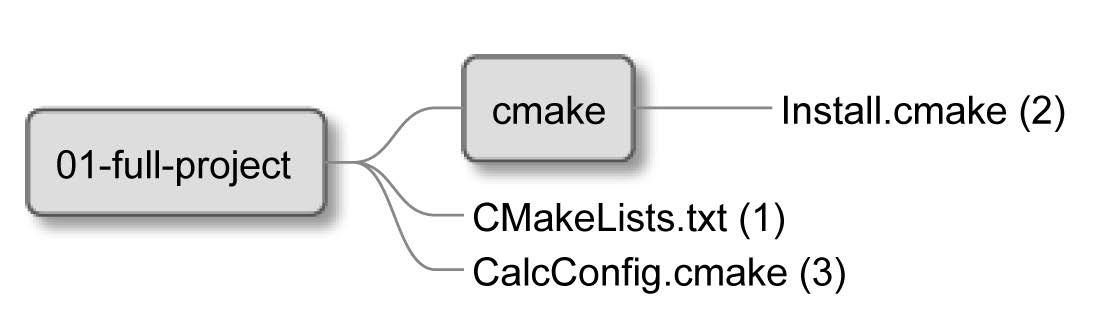
\includegraphics[width=0.8\textwidth]{content/3/chapter12/images/6.jpg}\\
Figure 12.6 – Files configuring installation and packaging
\end{center}

Only files are needed here – most of the work is already done in previous sections. As you may remember, the top-level listfile includes a CMake module that's going to handle this process:

\begin{lstlisting}[style=styleCMake]
# chapter-12/01-full-project/CMakeLists.txt (fragment)

...
include(Install)
\end{lstlisting}

We're interested in installing two items:

\begin{itemize}
\item 
The Calc library artifacts: the static library, the shared library, and header files along with their target export file

\item 
The Calc console executable
\end{itemize}

The package definition config-file will only introduce library targets, as potential consuming projects won't depend on the executable.

After configuring the installation steps, we'll move on to the CPack configuration. The high-level overview of the Install module looks like this:

\begin{lstlisting}[style=styleCMake]
# chapter-12/01-full-project/cmake/Install.cmake (overview)

# Includes
# Installation of Calc library
# Installation of Calc Console executable
# Configuration of CPack
\end{lstlisting}

Everything is planned, so it's time to write an installation module for the library.

\subsubsubsection{12.6.1\hspace{0.2cm}Installation of the library}

To install the library, it's best to start by configuring logical targets and specifying the destination for their artifacts. To avoid providing paths manually, we'll be using default values provided by the GNUInstallDirs module. For modularity, we'll group the artifacts into components. The default installation will install all files, but you may choose to only install the runtime component and skip the development artifacts:

\begin{lstlisting}[style=styleCMake]
# chapter-12/01-full-project/cmake/Install.cmake (fragment)

include(GNUInstallDirs)
# Calc library
install(TARGETS calc_obj calc_shared calc_static
	EXPORT CalcLibrary
	ARCHIVE COMPONENT development
	LIBRARY COMPONENT runtime
	PUBLIC_HEADER DESTINATION
		${CMAKE_INSTALL_INCLUDEDIR}/calc
			COMPONENT runtime
)
\end{lstlisting}

During the installation, we'd like to register the shared library we copied with ldconfig:

\begin{lstlisting}[style=styleCMake]
# chapter-12/01-full-project/cmake/Install.cmake (continued)

if (UNIX)
	install(CODE "execute_process(COMMAND ldconfig)"
		COMPONENT runtime
	)
endif()
\end{lstlisting}

Having those steps prepared, we can make the library visible to other CMake projects by wrapping it in a reusable CMake package. We'll need to generate and install the target export file and the config-file that includes it:

\begin{lstlisting}[style=styleCMake]
# chapter-12/01-full-project/cmake/Install.cmake (continued)

install(EXPORT CalcLibrary
	DESTINATION ${CMAKE_INSTALL_LIBDIR}/calc/cmake
	NAMESPACE Calc::
	COMPONENT runtime
)
install(FILES "CalcConfig.cmake"
	DESTINATION ${CMAKE_INSTALL_LIBDIR}/calc/cmake
)
\end{lstlisting}

As we already know, for very simple packages, the config-file can be really minimal:

\begin{lstlisting}[style=styleCMake]
# chapter-12/01-full-project/CalcConfig.cmake\\

include("${CMAKE_CURRENT_LIST_DIR}/CalcLibrary.cmake")
\end{lstlisting}

That's it. The library will now be installed when you run cmake in -{}-install mode after building the solution. All that remains to be installed is the executable.

\subsubsubsection{12.6.2\hspace{0.2cm}Installation of the executable}

The installation of binary executables is the simplest step of all. We just need to use a single command:

\begin{lstlisting}[style=styleCMake]
# chapter-12/01-full-project/cmake/Install.cmake (continued)

# CalcConsole runtime
install(TARGETS calc_console
	RUNTIME COMPONENT runtime
)
\end{lstlisting}

And it's done! Let's move on to the last part of the configuration – packing.

\subsubsubsection{12.6.3\hspace{0.2cm}Packaging with CPack}

We can go wild and configure a vast multitude of supported package types; for this project, however, a basic configuration will be enough:

\begin{lstlisting}[style=styleCMake]
# chapter-12/01-full-project/cmake/Install.cmake (continued)

# CPack configuration
set(CPACK_PACKAGE_VENDOR "Rafal Swidzinski")
set(CPACK_PACKAGE_CONTACT "email@example.com")
set(CPACK_PACKAGE_DESCRIPTION "Simple Calculator")
include(CPack)
\end{lstlisting}

Such a minimal setup works well for standard archives, such as ZIP files. We can test the whole installation and packaging with a single command (the project has to be built beforehand):


\begin{lstlisting}[style=styleCMake]
# chapter-12/01-full-project/cmake/Install.cmake (continued)

# CPack configuration
set(CPACK_PACKAGE_VENDOR "Rafal Swidzinski")
set(CPACK_PACKAGE_CONTACT "email@example.com")
set(CPACK_PACKAGE_DESCRIPTION "Simple Calculator")
include(CPack)
\end{lstlisting}

Such a minimal setup works well for standard archives, such as ZIP files. We can test the whole installation and packaging with a single command (the project has to be built beforehand):

\begin{tcblisting}{commandshell={}}
# cpack -G TGZ -B packages
CPack: Create package using TGZ
CPack: Install projects
CPack: - Run preinstall target for: Calc
CPack: - Install project: Calc []
CPack: Create package
CPack: - package: /tmp/b/packages/Calc-1.0.0-Linux.tar.gz
generated.
\end{tcblisting}

This concludes the installation and packaging; the next order of business is documentation.










